\documentclass[handout]{beamer}
%==============================================================
% Common Beamer Preamble for Course Lectures: Training and Scaling Language Models
%==============================================================

\usepackage[utf8]{inputenc}
\usepackage[T1]{fontenc}
\usepackage{hyperref}
\usepackage{amsmath,amssymb,xcolor,multicol,booktabs,colortbl}
\usepackage{graphicx,listings}
\renewcommand{\figurename}{Figure.}
\renewcommand{\tablename}{Table.}

% ---- TikZ Libraries ----
\usepackage{tikz}
\usetikzlibrary{positioning,arrows.meta,shapes.geometric,calc,fit,backgrounds,decorations.pathreplacing}

% ---- Presentation defaults ----
\setbeamertemplate{navigation symbols}{}
\setbeamersize{text margin left=0.55cm,text margin right=0.55cm}
\setbeamerfont{title}{size=\LARGE,series=\bfseries}
\setbeamerfont{subtitle}{size=\large}

% ---- FontAwesome fallback ----
\IfFileExists{fontawesome5.sty}{%
  \usepackage{fontawesome5}%
}{%
  \providecommand{\faMicrochip}{}%
  \providecommand{\faComments}{}%
  \providecommand{\faTools}{}%
  \providecommand{\faCheckCircle}{}%
  \providecommand{\faExclamationTriangle}{}%
  \providecommand{\faImage}{}%
  \providecommand{\faRobot}{}%
  \providecommand{\faTerminal}{}%
  \providecommand{\faBook}{}%
  \providecommand{\faRedo}{}%
  \providecommand{\faLayerGroup}{}%
  \providecommand{\faCogs}{}%
  \providecommand{\faDatabase}{}%
  \providecommand{\faHdd}{}%
  \providecommand{\faNetworkWired}{}%
}

% ---- Theme Style and Semantic Colors ----
%==============================================================
% Centralized Semantic Color Definitions for LLMs Presentation
%==============================================================

% ---- Base Template / Theme Colors (Aligned with Palette B) ----
\definecolor{themenavy}{RGB}{22,70,102}       % Palette B primary cerulean: #164666
\definecolor{themeblue}{RGB}{22,70,102}       % Primary alias
\definecolor{primarylight}{RGB}{34,92,132}    % Primary light: #225c84
\definecolor{themeteal}{RGB}{0,159,176}       % Accent cyan-teal: #009fb0
\colorlet{main_color}{themenavy}
\colorlet{accent}{themeteal}

\definecolor{accentdark}{RGB}{0,108,120}      % Deep cyan-teal for contrast text
\definecolor{accentlight}{RGB}{56,178,214}    % Slate accent cyan: #38b2d6
\definecolor{leafred}{RGB}{197,93,61}         % Terracotta red for branches/leaves

% ---- Website Panel & Border Neutrals ----
\definecolor{panelbg}{RGB}{237,245,249}       % Course-panel: #edf5f9
\definecolor{panelborder}{RGB}{204,226,238}   % Course-border: #cce2ee

% ---- Code listing style (syntax highlights) ----
\definecolor{deepblue}{RGB}{22,70,102}
\definecolor{deepred}{rgb}{0.6,0,0}
\definecolor{deepgreen}{RGB}{0,135,150}
\definecolor{halfgray}{gray}{0.55}

% ---- Semantic Theme Navy / Cerulean Shades ----
\colorlet{themebluebg}{panelbg}               % Panel #edf5f9
\colorlet{themebluecard}{main_color!8}        % Mild card background fills
\colorlet{themeblueborder}{panelborder}       % Border #cce2ee
\colorlet{themebluemid}{themeteal!60}         % Accent mid-contrast
\colorlet{themebluedraw}{main_color!80}       % Strong outline draws/strokes

% ---- Semantic Secondary Accent Teal Shades ----
\colorlet{accentdarkbg}{themeteal!10}        % Light secondary background fills
\colorlet{accentdarkdraw}{themeteal}         % Secondary outlines/strokes/text/axes

% ---- Functional Colors: Success Green ----
\definecolor{successgreen}{RGB}{55,145,55}
\colorlet{successbg}{successgreen!8}
\colorlet{successdraw}{successgreen!75}

% ---- Functional Colors: Alert Red ----
\definecolor{alertred}{RGB}{197,55,55}
\colorlet{alertbg}{alertred!8}
\colorlet{alertdraw}{alertred!75}

% ---- Functional Colors: Warning Orange ----
\definecolor{warningorange}{RGB}{220,110,30}
\colorlet{warningbg}{warningorange!10}
\colorlet{warningdraw}{warningorange!80}

% ---- Terracotta Red Shades ----
\colorlet{leafredbg}{leafred!12}
\colorlet{leafreddraw}{leafred!80}

% ---- Accent Violet (SWE-bench / observe phases) ----
\definecolor{accentviolet}{RGB}{120,70,180}
\colorlet{accentvioletbg}{accentviolet!10}
\colorlet{accentvioletdraw}{accentviolet!80}

% ---- Post-Training Axis Blue ----
\definecolor{posttrainingblue}{RGB}{40,90,165}
\colorlet{posttrainingbg}{posttrainingblue!8}
\colorlet{posttrainingdraw}{posttrainingblue!75}

% ---- Harness Component Action Green ----
\definecolor{actiongreen}{RGB}{55,145,55}
\colorlet{actiongreenbg}{actiongreen!10}
\colorlet{actiongreendraw}{actiongreen!65}

% ---- Harness Component Persist Olive ----
\definecolor{persistolive}{RGB}{120,135,40}
\colorlet{persistolivebg}{persistolive!12}
\colorlet{persistolivedraw}{persistolive!70}

% ---- Harness Component Observe Violet ----
\colorlet{observevioletbg}{accentvioletbg}
\colorlet{observevioletdraw}{accentvioletdraw}

% ---- Neutrals (Grays/Blacks) ----
\colorlet{neutralbg}{black!4}             % Very light background fills
\colorlet{neutrallight}{black!30}         % Border frames/ticks/dividers
\colorlet{neutraldark}{black!75}          % Main body text/code listing text

% ---- Beamer Block Color Overrides (Premium Terracotta Theme) ----
\setbeamercolor{block title alert}{bg=leafreddraw,fg=white}
\setbeamercolor{block body alert}{bg=leafredbg}
\setbeamercolor{alerted text}{fg=leafreddraw}

\usepackage{../common/style}
\graphicspath{{../common/figs/}{figs/}}

% ---- Code Listing Config ----
\lstset{
  basicstyle=\ttfamily\footnotesize,
  keywordstyle=\bfseries\color{deepblue},
  emphstyle=\ttfamily\color{deepred},
  stringstyle=\color{deepgreen},
  commentstyle=\color{halfgray}\itshape,
  numbers=left, numberstyle=\tiny\color{halfgray},
  backgroundcolor=\color{codebg},
  frame=l, framerule=1.5pt, rulecolor=\color{themeteal},
  xleftmargin=10pt, framexleftmargin=4pt, numbersep=6pt,
  showstringspaces=false, breaklines=true,
  aboveskip=4pt, belowskip=4pt
}

% ---- Image Placeholder Utility ----
\newcommand{\slideimage}[2][3.8cm]{%
  \begin{center}
    \begin{tikzpicture}
      \node[draw=main_color, dashed, very thick, rounded corners,
        fill=themebluebg, minimum width=0.88\linewidth, minimum height=#1,
      text width=0.80\linewidth, align=center, font=\itshape, text=accentdark]
      {\textbf{[ FIGURE / DIAGRAM ]}\\[6pt] #2};
    \end{tikzpicture}
  \end{center}
}

% ---- Concept Highlight Card Utility ----
\newcommand{\conceptcard}[3]{%
  \begin{coursebox}{#1}{#2}#3
  \end{coursebox}%
}

% ---- Reusable teaching-slide components ----
\newcommand{\learninggoals}[4]{%
  \begin{frame}{What should be clear by the end?}
    \begin{enumerate}
        \setlength{\itemsep}{7pt}
      \item #1
      \item #2
      \item #3
      \item #4
    \end{enumerate}
  \end{frame}
}

\newcommand{\checkpoint}[2]{%
  \begin{frame}{Checkpoint: #1}
    \begin{block}{Think, then compare}
      #2
    \end{block}
  \end{frame}
}

\newcommand{\takeaways}[4]{%
  \begin{frame}{Key takeaways}
    \begin{enumerate}
        \setlength{\itemsep}{8pt}
      \item #1
      \item #2
      \item #3
      \item #4
    \end{enumerate}
  \end{frame}
}

\newcommand{\smallsource}[1]{%
  \vfill\hfill{\tiny\color{neutraldark}Source: #1}
}

% ---- Logo on content frames ----
\newif\ifplacelogo
\placelogotrue
\logo{\ifplacelogo
  \raisebox{-0.3ex}{
\includegraphics[height=0.4cm]{IMT_Atlantique_logo.png}}%
\fi}

\makeatletter
\define@key{beamerframe}{nologo}[true]{%
  \placelogofalse
}
\makeatother

% Fix Beamer bold font warning: substitute undefined T1/cmss/b/n with T1/cmss/bx/n
\DeclareFontShape{T1}{cmss}{b}{n}{<->ssub * cmss/bx/n}{}

% Default Author, Institute & Date metadata
\author[BRAIN team]{BRAIN team}
\institute[IMT Atlantique]{IMT Atlantique}
\date{January 2027}

% Override \date so individual decks calling \date{\today} do not overwrite the common date
\renewcommand{\date}[2][]{}

% ---- Front Page / Title Slide Macro ----
% Displays Title + IMT Atlantique logo and Brain logo
\newcommand{\makelecturetitle}[1][Training and Scaling Language Models: From First Principles to Efficient Serving]{%
  \placelogofalse
  {
    \setbeamertemplate{footline}{}
    \settitletagline{#1}
    \settitlelogos{%
      \raisebox{-0.5\height}{
\includegraphics[height=1.15cm]{IMT_Atlantique_logo.png}}%
      \hspace{1.2em}%
    \raisebox{-0.5\height}{\includegraphics[height=1.15cm]{brain.pdf}}}
    \def\insertauthor{BRAIN team}
    \def\insertdate{January 2027}
    \begin{frame}[plain]
      \titlepage
    \end{frame}
  }
  \placelogotrue
}

% Section TOC Frame
\AtBeginSection[]{\coursesectiondivider}

\title[TASLLM -- Module 10]{Module 10: Serving Systems\\[4pt]
\normalsize\itshape Scheduling Tokens under Latency and Memory Constraints}
\date{\today}

\begin{document}
\makelecturetitle
\begin{frame}{Lecture map}
  \tableofcontents
  \vfill
  \begin{block}{Guiding question}
    How does an inference engine turn irregular requests into efficient GPU work while protecting latency objectives?
  \end{block}
\end{frame}
\learninggoals
{Trace a request through scheduler, cache manager, model runner, and output path.}
{Explain continuous batching and chunked prefill at iteration granularity.}
{Connect paged KV memory, admission control, and preemption.}
{Design a serving benchmark with explicit workload and latency metrics.}

\section{From model forward to inference engine}

\begin{frame}{One engine iteration: from requests to GPU and back}
  \centering
  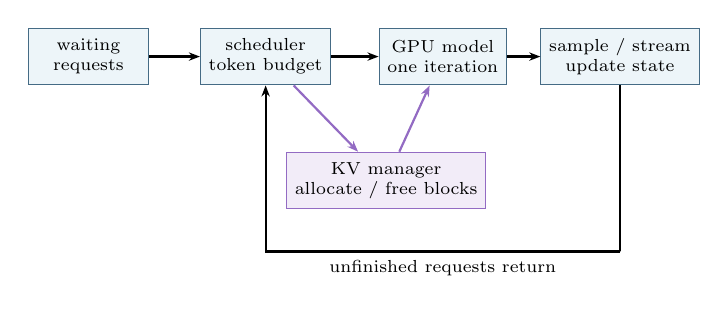
\begin{tikzpicture}[x=1cm,y=1cm,scale=.9,transform shape,every node/.style={font=\scriptsize,align=center},
    box/.style={draw=themebluedraw,fill=themebluebg,minimum width=1.7cm,minimum height=.8cm},
    cache/.style={draw=accentvioletdraw,fill=accentvioletbg,minimum width=2.2cm,minimum height=.8cm},
    arrow/.style={-{Stealth[length=4pt]},thick}]
    \node[box] (queue) at (0,2) {waiting\\requests};
    \node[box] (scheduler) at (2.5,2) {scheduler\\token budget};
    \node[box] (runner) at (5,2) {GPU model\\one iteration};
    \node[box] (sampler) at (7.5,2) {sample / stream\\update state};
    \node[cache] (cache) at (4.2,.25) {KV manager\\allocate / free blocks};
    \draw[arrow] (queue)--(scheduler); \draw[arrow] (scheduler)--(runner); \draw[arrow] (runner)--(sampler);
    \draw[arrow,accentvioletdraw] (scheduler)--(cache); \draw[arrow,accentvioletdraw] (cache)--(runner);
    \draw[arrow] (sampler.south) |- (7.5,-.75) -| node[pos=.25,below]{unfinished requests return} (scheduler.south);
  \end{tikzpicture}
  \par\vspace{5pt}\small At each iteration, choose token work, reserve cache space, run the model, then stream outputs and retire finished requests.
\end{frame}

\begin{frame}{Prefill and decode compete for the same device}
  \begin{columns}[t]
    \begin{column}{0.47\linewidth}
      \begin{block}{Prefill request}
        many prompt tokens\\high parallelism\\large temporary attention work\\drives time to first token
      \end{block}
    \end{column}
    \begin{column}{0.47\linewidth}
      \begin{block}{Decode request}
        one token per active sequence\\growing KV reads\\latency sensitive\\drives inter-token latency
      \end{block}
    \end{column}
  \end{columns}
  \begin{alertblock}{Scheduling tension}
    A long prefill can increase throughput but block many decode tokens, causing visible latency spikes.
  \end{alertblock}
\end{frame}

\begin{frame}{Speculative decoding}
  \centering
  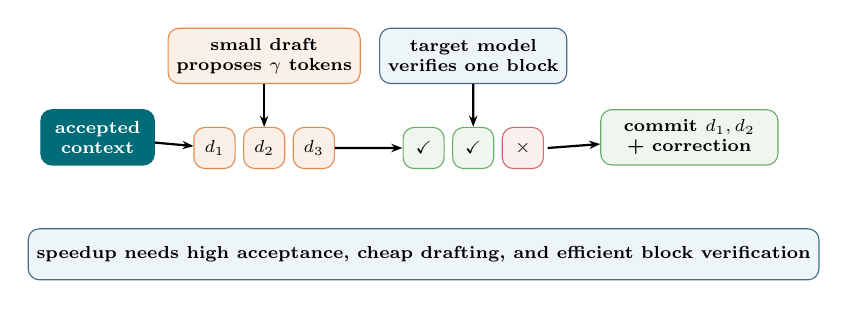
\begin{tikzpicture}[x=1cm,y=1cm,scale=.90,transform shape,every node/.style={font=\scriptsize},
      stage/.style={rounded corners,minimum height=.78cm,align=center,font=\scriptsize\bfseries},
    token/.style={rounded corners,minimum width=.58cm,minimum height=.58cm,font=\scriptsize\bfseries}]
    \node[stage,draw=accentdark,fill=accentdark,text=white,minimum width=1.6cm] (ctx) at (.8,2.4) {accepted\\context};
    \node[stage,draw=warningdraw,fill=warningbg,minimum width=1.9cm] (draft) at (3.15,3.55) {small draft\\proposes $\gamma$ tokens};
    \node[token,draw=warningdraw,fill=warningbg] (d1) at (2.45,2.25) {$d_1$};
    \node[token,draw=warningdraw,fill=warningbg] (d2) at (3.15,2.25) {$d_2$};
    \node[token,draw=warningdraw,fill=warningbg] (d3) at (3.85,2.25) {$d_3$};
    \node[stage,draw=themebluedraw,fill=themebluebg,minimum width=2.1cm] (target) at (6.1,3.55) {target model\\verifies one block};
    \node[token,draw=successdraw,fill=successbg] at (5.4,2.25) {$\checkmark$};
    \node[token,draw=successdraw,fill=successbg] at (6.1,2.25) {$\checkmark$};
    \node[token,draw=alertdraw,fill=alertbg] at (6.8,2.25) {$\times$};
    \node[stage,draw=successdraw,fill=successbg,minimum width=2.5cm] (commit) at (9.15,2.4) {commit $d_1,d_2$\\+ correction};
    \draw[-{Stealth[length=4pt,width=3pt]},thick] (ctx)--(d1);
    \draw[-{Stealth[length=4pt,width=3pt]},thick] (draft.south)--(d2.north);
    \draw[-{Stealth[length=4pt,width=3pt]},thick] (d3)--(5.1,2.25);
    \draw[-{Stealth[length=4pt,width=3pt]},thick] (target.south)--(6.1,2.55);
    \draw[-{Stealth[length=4pt,width=3pt]},thick] (7.15,2.25)--(commit);
    \node[draw=themebluedraw,fill=themebluebg,rounded corners,minimum width=8.4cm,minimum height=.72cm,align=center,font=\scriptsize\bfseries] at (5.4,.75)
    {speedup needs high acceptance, cheap drafting, and efficient block verification};
  \end{tikzpicture}
  \par\vspace{2pt}
  \footnotesize Correct rejection sampling preserves the target distribution; measure accepted tokens per target step and TPOT.\par
  \smallsource{MVA Training and Deploying Large-Scale Models, Lecture 6 (2026)}
\end{frame}

\begin{frame}{Static batching waits for the slowest request}
  \begin{center}
    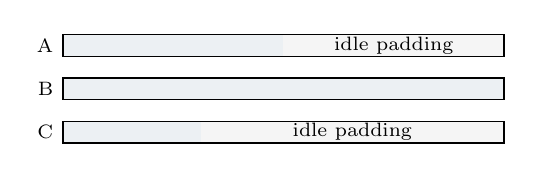
\begin{tikzpicture}[x=.7cm,y=.55cm,every node/.style={font=\scriptsize}]
      \foreach \y/\name in {3/A,2/B,1/C}{\node[left] at (0,\y+.25) {\name};}
      \fill[themebluecard] (0,3) rectangle (4,3.5);
      \fill[neutralbg] (4,3) rectangle (8,3.5);
      \fill[themebluecard] (0,2) rectangle (8,2.5);
      \fill[themebluecard] (0,1) rectangle (2.5,1.5);
      \fill[neutralbg] (2.5,1) rectangle (8,1.5);
      \draw (0,3) rectangle (8,3.5); \draw (0,2) rectangle (8,2.5); \draw (0,1) rectangle (8,1.5);
      \node at (6,3.25) {idle padding}; \node at (5.25,1.25) {idle padding};
    \end{tikzpicture}
  \end{center}
  \begin{alertblock}{Head-of-line effect}
    Completed sequences occupy batch slots until the longest member finishes. New work cannot enter even when capacity is available.
  \end{alertblock}
\end{frame}

\begin{frame}{Continuous batching repacks every iteration}
  \centering
  \begin{tikzpicture}[x=.72cm,y=.56cm,every node/.style={font=\scriptsize}]
    \node[anchor=west,font=\scriptsize\bfseries] at (2.2,6.65) {static batch};
    \node[anchor=west,font=\scriptsize\bfseries,text=accentdark] at (2.2,2.85) {continuous batch};
    \foreach \x in {0,...,7}{\node[text=neutraldark] at (2.6+\x,6.15) {\pgfmathparse{int(\x+1)}\pgfmathresult};}
    \foreach \y/\name in {5.4/A,4.55/B,3.7/C}{\node[left] at (2.05,\y+.25) {\name};}
    \foreach \x in {0,1,2}{\fill[themebluedraw] (2.2+\x,5.4) rectangle (3.2+\x,5.9);}
    \fill[neutralbg] (5.2,5.4) rectangle (10.2,5.9); \node at (7.7,5.65) {idle};
    \foreach \x in {0,...,7}{\fill[themebluedraw] (2.2+\x,4.55) rectangle (3.2+\x,5.05);}
    \foreach \x in {0,1}{\fill[themebluedraw] (2.2+\x,3.7) rectangle (3.2+\x,4.2);}
    \fill[neutralbg] (4.2,3.7) rectangle (10.2,4.2); \node at (7.2,3.95) {idle};
    \draw[neutrallight] (2.2,3.7) rectangle (10.2,5.9);
    \draw[neutrallight] (2.2,3.7)--(10.2,3.7); \draw[neutrallight] (2.2,4.55)--(10.2,4.55); \draw[neutrallight] (2.2,5.4)--(10.2,5.4);
    \foreach \y/\name in {1.9/slot 1,1.05/slot 2,.2/slot 3}{\node[left] at (2.05,\y+.25) {\name};}
    \foreach \x in {0,1,2}{\fill[themebluedraw] (2.2+\x,1.9) rectangle (3.2+\x,2.4);}
    \fill[signaldark] (5.2,1.9) rectangle (6.2,2.4); \node[text=white,font=\tiny\bfseries] at (5.7,2.15) {D};
    \foreach \x in {4,5,6,7}{\fill[themebluedraw] (2.2+\x,1.9) rectangle (3.2+\x,2.4);}
    \foreach \x in {0,...,7}{\fill[themebluedraw] (2.2+\x,1.05) rectangle (3.2+\x,1.55);}
    \foreach \x in {0,1}{\fill[themebluedraw] (2.2+\x,.2) rectangle (3.2+\x,.7);}
    \fill[signaldark] (4.2,.2) rectangle (5.2,.7); \node[text=white,font=\tiny\bfseries] at (4.7,.45) {E};
    \foreach \x in {3,4,5,6,7}{\fill[themebluedraw] (2.2+\x,.2) rectangle (3.2+\x,.7);}
    \draw[neutrallight] (2.2,.2) rectangle (10.2,2.4);
    \foreach \x in {0,...,7}{\draw[white] (2.2+\x,.2)--(2.2+\x,2.4);}
    \node[anchor=west,draw=successdraw,fill=successbg,rounded corners,align=center,font=\tiny\bfseries] at (10.5,1.3) {orange: prefill\\blue: decode};
  \end{tikzpicture}
  \vspace{3pt}
  \begin{block}{Scheduling unit}
    Repack useful decode tokens and prefill chunks every step, subject to token and KV-block budgets.
  \end{block}
\end{frame}

\section{Token and memory scheduling}

\begin{frame}{A token budget bounds work per engine step}
  Suppose the iteration budget is $N_{\max}$ scheduled tokens.
  \[
    N_{\text{decode}}+N_{\text{prefill}}\le N_{\max}
  \]
  \begin{itemize}
      \setlength{\itemsep}{8pt}
    \item Every active decode sequence usually asks for one token.
    \item Remaining capacity can admit prompt tokens.
    \item Cache-block availability may be the tighter constraint.
  \end{itemize}
  \begin{alertblock}{Policy matters}
    Prioritizing decode protects inter-token latency. Prioritizing large prefills may improve throughput but delay active users.
  \end{alertblock}
\end{frame}

\begin{frame}{Chunked prefill shares iterations with decode}
  \centering
  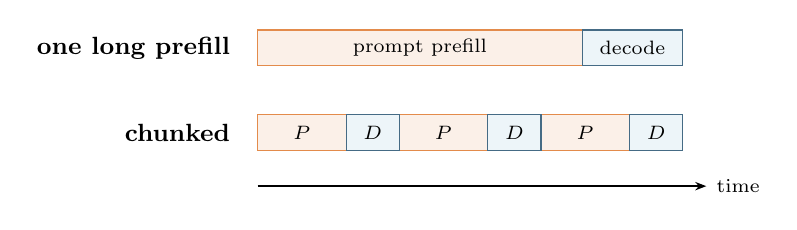
\begin{tikzpicture}[x=.75cm,y=.65cm,every node/.style={font=\scriptsize,align=center}]
    \node[anchor=east,font=\small\bfseries] at (-.3,2.8) {one long prefill};
    \node[anchor=east,font=\small\bfseries] at (-.3,1.15) {chunked};
    \fill[warningbg,draw=warningdraw] (0,2.45) rectangle (5.5,3.15); \node at (2.75,2.8) {prompt prefill};
    \fill[themebluebg,draw=themebluedraw] (5.5,2.45) rectangle (7.2,3.15); \node at (6.35,2.8) {decode};
    \foreach \x in {0,2.4,4.8}{\fill[warningbg,draw=warningdraw] (\x,.8) rectangle (\x+1.5,1.5); \node at (\x+.75,1.15) {$P$};}
    \foreach \x in {1.5,3.9,6.3}{\fill[themebluebg,draw=themebluedraw] (\x,.8) rectangle (\x+.9,1.5); \node at (\x+.45,1.15) {$D$};}
    \draw[-{Stealth[length=4pt]},thick] (0,.1)--(7.6,.1) node[right]{time};
  \end{tikzpicture}
  \par\vspace{4pt}
  \small P: prefill chunk; D: decode for other active requests. An iteration can mix both kinds of work, limiting long decode stalls.
  \begin{alertblock}{Trade-off}
    Smaller chunks can reduce blocking but add scheduling/launch overhead and may lower prefill efficiency. The prompt must complete before its first generated token.
  \end{alertblock}
\end{frame}

\begin{frame}{Paged KV: logical tokens map to physical blocks}
  \centering
  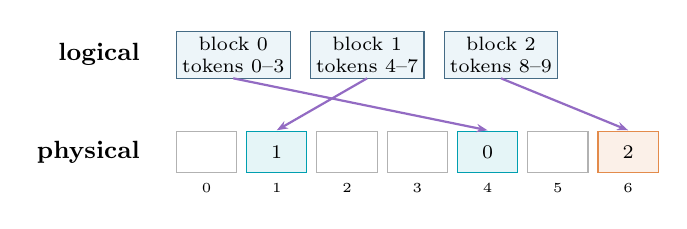
\begin{tikzpicture}[x=.85cm,y=.75cm,every node/.style={font=\scriptsize,align=center}]
    \node[anchor=east,font=\small\bfseries] at (-.4,3) {logical};
    \foreach \i/\label in {0/{0--3},1/{4--7},2/{8--9}}{
      \fill[themebluebg,draw=themebluedraw] (\i*2,2.6) rectangle (\i*2+1.7,3.4);
      \node at (\i*2+.85,3) {block \i\\tokens \label}; }
    \node[anchor=east,font=\small\bfseries] at (-.4,1.35) {physical};
    \foreach \i in {0,...,6}{\draw[neutrallight] (\i*1.05,1) rectangle (\i*1.05+.9,1.7); \node[font=\tiny] at (\i*1.05+.45,.75) {\i};}
    \fill[accentdarkbg,draw=accentdarkdraw] (4.2,1) rectangle (5.1,1.7); \node at (4.65,1.35) {0};
    \fill[accentdarkbg,draw=accentdarkdraw] (1.05,1) rectangle (1.95,1.7); \node at (1.5,1.35) {1};
    \fill[warningbg,draw=warningdraw] (6.3,1) rectangle (7.2,1.7); \node at (6.75,1.35) {2};
    \draw[-{Stealth[length=4pt]},thick,accentvioletdraw] (.85,2.6)--(4.65,1.72);
    \draw[-{Stealth[length=4pt]},thick,accentvioletdraw] (2.85,2.6)--(1.5,1.72);
    \draw[-{Stealth[length=4pt]},thick,accentvioletdraw] (4.85,2.6)--(6.75,1.72);
  \end{tikzpicture}
  \par\vspace{4pt}
  \small Block table: $[4,1,6]$. With four token slots per block, ten cached tokens use three blocks; the last has two unused slots.
  \par\footnotesize Conceptual blocks represent the KV storage for a token range; actual layouts organize layers and devices differently.
\end{frame}

\begin{frame}{Explore batching and paged allocation}
  \begin{block}{Interactive serving simulator}
    \href{https://brain-bzh.github.io/llm-course/demos/continuous-batching.html}{\textbf{Open the batching and paged-KV demo} $\nearrow$}
  \end{block}
  \begin{enumerate}
    \item Compare static and continuous batching under the same arrivals.
    \item Step through a request's logical-to-physical block table as it grows and finishes.
    \item Change prompt lengths, block size and token budget; compare TTFT and occupancy.
  \end{enumerate}
  \small This is a teaching simulation: validate scheduling and performance claims on the target engine and hardware.
\end{frame}

\begin{frame}{Prefix caching trades index work for avoided prefill}
  A cache hit can reuse KV blocks for an identical token prefix.
  \begin{columns}[t]
    \begin{column}{0.47\linewidth}
      \begin{block}{Works well for}
        repeated system prompts\\shared document prefixes\\branching completions
      \end{block}
    \end{column}
    \begin{column}{0.47\linewidth}
      \begin{alertblock}{Correctness conditions}
        identical model and adapter\\identical token IDs and positions\\compatible cache precision and layout
      \end{alertblock}
    \end{column}
  \end{columns}
  Measure hit rate, tokens avoided, retained-block cost, and eviction behavior together.
\end{frame}

\begin{frame}{Admission control prevents memory collapse}
  Before admitting work, estimate required blocks from prompt length, current cache, and maximum generation policy.
  \begin{itemize}
      \setlength{\itemsep}{7pt}
    \item queue when safe cache capacity is unavailable
    \item reject or cap requests outside the service contract
    \item preempt lower-priority work only under a declared policy
    \item distinguish recomputation preemption from host-memory swapping
  \end{itemize}
  \begin{alertblock}{Overcommit is not free}
    Preemption can recover capacity but adds wasted compute, extra latency, and tail-risk amplification.
  \end{alertblock}
\end{frame}

\begin{frame}{CUDA graphs reward stable execution shapes}
  Capturing a repeated GPU execution removes CPU launch overhead, but dynamic batches change shapes and memory addresses.
  \begin{columns}[t]
    \begin{column}{0.47\linewidth}
      \begin{block}{Engine strategy}
        capture a set of padded batch shapes\\reuse stable buffers\\fall back for unsupported shapes
      \end{block}
    \end{column}
    \begin{column}{0.47\linewidth}
      \begin{alertblock}{Trade-off}
        More capture sizes reduce padding but consume memory and operational complexity.
      \end{alertblock}
    \end{column}
  \end{columns}
\end{frame}

\checkpoint{schedule by hand}
{An iteration budget is 16 tokens. Ten sequences need decode, one waiting prompt has length 20, and cache capacity is available. Propose the next two iterations under a decode-first chunked-prefill policy.}

\section{Measure the service, not a toy loop}

\begin{frame}{A request has several latency clocks}
  \centering
  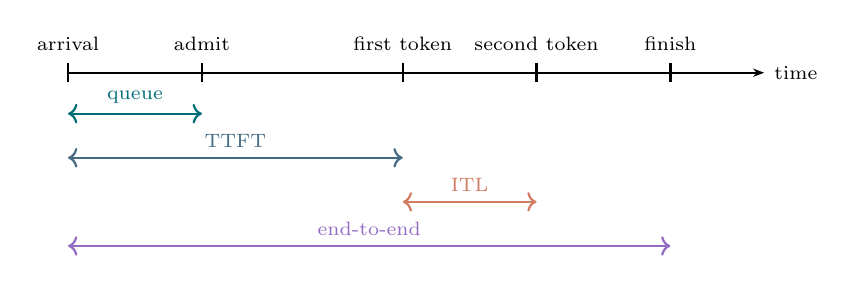
\begin{tikzpicture}[x=.85cm,y=.8cm,every node/.style={font=\scriptsize,align=center}]
    \draw[-{Stealth[length=4pt]},thick] (0,1)--(10.4,1) node[right]{time};
    \foreach \x/\lab in {0/arrival,2/admit,5/first token,7/second token,9/finish}{
      \draw[thick] (\x,.85)--(\x,1.15); \node[above] at (\x,1.2) {\lab}; }
    \draw[<->,thick,accentdark] (0,.35)--node[above]{queue}(2,.35);
    \draw[<->,thick,themebluedraw] (0,-.35)--node[above]{TTFT}(5,-.35);
    \draw[<->,thick,leafreddraw] (5,-1.05)--node[above]{ITL}(7,-1.05);
    \draw[<->,thick,accentvioletdraw] (0,-1.75)--node[above]{end-to-end}(9,-1.75);
  \end{tikzpicture}
  \par\vspace{6pt}
  \small TTFT includes queueing and prefill; ITL is one gap between streamed tokens. TPOT often summarizes the mean gap per request.
  \begin{block}{Service goal}
    Report throughput alongside p50/p95/p99 latency; goodput counts requests satisfying the declared latency objectives.
  \end{block}
\end{frame}

\begin{frame}{Open-loop and closed-loop loads answer different questions}
  \begin{columns}[t]
    \begin{column}{0.47\linewidth}
      \begin{block}{Closed loop}
        Each client waits for completion before sending again. Offered load falls automatically when the server slows.
      \end{block}
    \end{column}
    \begin{column}{0.47\linewidth}
      \begin{block}{Open loop}
        Arrivals follow an external process. Queues grow when demand exceeds capacity, revealing overload behavior.
      \end{block}
    \end{column}
  \end{columns}
  \begin{alertblock}{Benchmark declaration}
    Report arrival process, prompt and output distributions, sampling settings, concurrency, warmup, and duration.
  \end{alertblock}
\end{frame}

\begin{frame}{A useful benchmark sweeps the operating curve}
  \begin{enumerate}
      \setlength{\itemsep}{7pt}
    \item choose a representative request-length distribution
    \item increase arrival rate or concurrency gradually
    \item record TTFT, inter-token latency, throughput, cache occupancy, and preemptions
    \item identify the saturation knee and tail-latency cliff
    \item compare policies at matched service-level objectives
  \end{enumerate}
  \begin{block}{The right conclusion}
    ``Policy A delivers more tokens/s while keeping p99 TTFT below the declared threshold for workload W.''
  \end{block}
\end{frame}

\begin{frame}{Read metrics as one coupled system}
  \begin{itemize}
      \setlength{\itemsep}{7pt}
    \item rising queue time with stable GPU time means admission is saturated
    \item TTFT spikes with stable decode latency suggest long prefills or queueing
    \item growing preemptions suggest cache overcommit
    \item high cache occupancy with low throughput suggests bandwidth or scheduler inefficiency
    \item lower mean latency with worse p99 may indicate unfair prioritization
  \end{itemize}
\end{frame}

\checkpoint{serving report}
{Define a workload, one service-level objective, the policy under test, a baseline, and the five measurements needed to explain both throughput and tail latency.}

\takeaways
{An inference engine schedules token work and cache state at every iteration.}
{Continuous batching removes static slots, while chunked prefill controls head-of-line blocking.}
{Paged memory, prefix reuse, admission, and preemption jointly determine capacity.}
{Serving claims require representative arrivals plus throughput and tail-latency evidence.}
\end{document}
